\documentclass[11pt]{article}

% --------------------
% Packages
% --------------------
\usepackage[margin=1in]{geometry}
\usepackage{amsmath, amssymb, amsfonts}
\usepackage{graphicx}
\usepackage{float}
\usepackage{caption}
\usepackage{booktabs}
\usepackage{enumitem}
\usepackage{mathtools}
\usepackage{hyperref}
\usepackage{helvet}
\renewcommand{\familydefault}{\sfdefault}

\setlength{\parindent}{0in}

% --------------------
% Formatting
% --------------------
\title{Numerical PDEs Homework \#1}
\author{Hope Elsayed}
\date{10/6/26}

\begin{document}

\maketitle

% ==================================================
\section*{Stokes Equations - Setup}
% ==================================================

Consider the two-dimensional Stokes equations
\begin{align*}
    \mu \nabla^2 \mathbf{u} - \nabla P &= \mathbf{b}, \\
    \nabla \cdot \mathbf{u} &= 0,
\end{align*}
where
\[ \mathbf{u} =
\begin{bmatrix}
U \\ V
\end{bmatrix},
\qquad
\mathbf{b} =
\begin{bmatrix}
f \\ g
\end{bmatrix},
\qquad
\mu = 1.
\]

Periodic boundary conditions are imposed in the $x$-direction. 
At the top and bottom boundaries,
\[
U = 0,
\qquad
V = -3.5.
\]
\newpage
% ==================================================
\section*{Problem 1: Manufactured Solution}
% ==================================================

Solve the Stokes equations using the manufactured solution
\begin{align*}
    U_{\mathrm{an}}(x,y) &= \sin(2\pi y)\sin(2\pi x), \\
    V_{\mathrm{an}}(x,y) &= -3.5
    + \cos(2\pi x)\left[\cos(2\pi y)-1\right], \\
    P_{\mathrm{an}}(x,y) &= \sin(2\pi y)\cos(2\pi x).
\end{align*}

Determine the right hand side functions $f(x,y)$ and $g(x,y)$ that force our solutions to fit these equations. Because pressure is nonunique up to an additive constant, subtract its mean before comparing the solutions. \\

\textbf{Solution: } \\
For the $U$ component of velocity, the second derivatives with respect to x and y are
\begin{align*}
    U_{xx} &= -4\pi^2\sin(2\pi y)\sin(2\pi x), \\
    U_{yy} &= -4\pi^2\sin(2\pi y)\sin(2\pi x),
\end{align*}
so the Laplacian is
\[
    \nabla^2 U
    = -8\pi^2\sin(2\pi y)\sin(2\pi x).
\] \\

For the $V$ component of velocity, the second derivatives with respect to x and y are
\begin{align*}
    V_{xx}&= -4\pi^2\cos(2\pi x)\left[\cos(2\pi y)-1\right], \\
    V_{yy}&= -4\pi^2\cos(2\pi x)\cos(2\pi y),
\end{align*}
so the Laplacian is
\begin{align*}
    \nabla^2 V
    &= -4\pi^2\cos(2\pi x) \left[2\cos(2\pi y)-1\right].
\end{align*} \\


The pressure derivatives with respect to x and y are
\begin{align*}
    P_x &= -2\pi\sin(2\pi y)\sin(2\pi x), \\
    P_y &= 2\pi\cos(2\pi y)\cos(2\pi x).
\end{align*} \\

Therefore, the right hand side becomes
\begin{align*}
    f(x,y) &= \nabla^2 U-P_x \\
    &= (-8\pi^2+2\pi) \sin(2\pi y)\sin(2\pi x), \\
    g(x,y)&= \nabla^2 V-P_y \\
    &= \left[-8\pi^2\cos(2\pi y)+4\pi^2-2\pi\cos(2\pi y)\right]\cos(2\pi x).
\end{align*}



The manufactured solution satisfies the incompressibility condition. The derivatives are
\begin{align*}
    U_x &= 2\pi\sin(2\pi y)\cos(2\pi x), \\
    V_y &= -2\pi\cos(2\pi x)\sin(2\pi y).
\end{align*}

So, we can see that
\[
    \nabla\cdot\mathbf{u}
    = U_x+V_y
    = 0.
\] 

\begin{figure}[H]
    \centering
    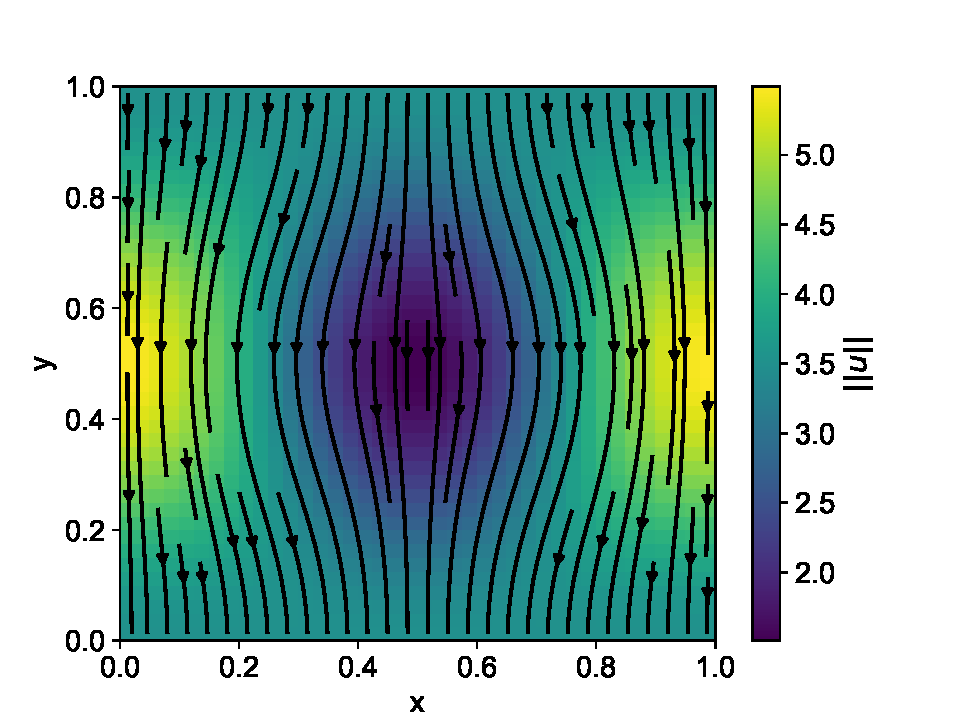
\includegraphics[width=0.8\textwidth]{velocity.pdf}
    \caption{Numerical velocity magnitude $\|\mathbf{u}\|$ and velocity
    field for $N_x=N_y=40$.}
    \label{fig:velocity}
\end{figure}

Using these functions, the Stokes system was discretized on a staggered grid using centered finite differences and solved using a direct sparse solver. Figure~\ref{fig:velocity} shows the resulting velocity magnitude and velocity field for $N_x=N_y=40$.

\newpage
% ==================================================
\section*{Problem 2: Convergence}
% ==================================================

Repeat for increasing grid sizes $N_x=N_y=N$. Compute the relative $L_2$ errors and show that we see second-order error decreases in our numerical solution $\left( U_{num}\right)$ compared to our analytical solution $\left( U_{an}\right)$. The error is calculated using the following norm equation:
\[
    \mathrm{err}_U =
    \frac{\|U_{\mathrm{num}}-U_{\mathrm{an}}\|_2}
         {\|U_{\mathrm{an}}\|_2}.
\] \\

\textbf{Solution: } \\
The Stokes equation was solved using increasing grid sizes $N_x=N_y=N$ for $N=$ 10, 20, 30, 40, and 50. At each grid size, the numerical solutions were compared with the analytic solutions. The relative $L_2$ errors were calculated as
\begin{align*}
    \mathrm{err}_U &=
    \frac{\|U_{\mathrm{num}}-U_{\mathrm{an}}\|_2}
         {\|U_{\mathrm{an}}\|_2}, \\
    \mathrm{err}_V &=
    \frac{\|V_{\mathrm{num}}-V_{\mathrm{an}}\|_2}
         {\|V_{\mathrm{an}}\|_2}, \\
    \mathrm{err}_P &=
    \frac{\|P_{\mathrm{num}}-P_{\mathrm{an}}\|_2}
         {\|P_{\mathrm{an}}\|_2}.
\end{align*}

Because adding a constant to pressure gives a solution, the mean was subtracted from both the numerical and analytic pressure solutions before calculating the pressure error. 

\begin{figure}[H]
    \centering
    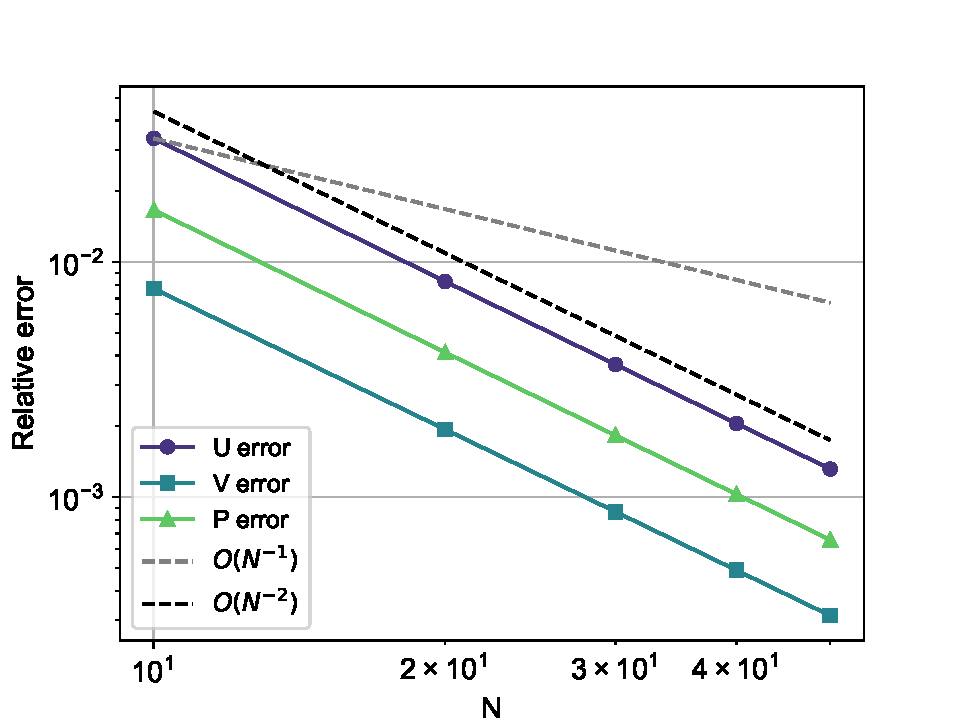
\includegraphics[width=0.8\textwidth]{relative_error.pdf}
    \caption{Relative $L_2$ errors in $U$, $V$, and $P$ with
    first- and second-order reference rates.}
    \label{fig:relative_error}
\end{figure}

Figure~\ref{fig:relative_error} shows that the relative errors in $U$, $V$, and $P$ all decrease as the grid size increases. The errors all decrease following the $O(N^{-2})$ reference line rather than the $O(N^{-1})$ line. Therefore, the numerical solution demonstrates an approximate second-order convergence, which makes sense as we used centered finite difference approximations. 


\newpage
% ==================================================
\section*{Problem 3: GMRES}
% ==================================================

You should never just stop once you have a cool code. The best part is to play around with it. So do something fun with your code and show it off! \\

\textbf{Solution: } \\
For the third problem, I compared the compute time of the direct sparse solver with the iterative GMRES solver for increasing grid sizes. The time required to construct the matrix and right hand side was not included. Only the solvers themselves were counted. \\

The Stokes equation was solved using increasing grid sizes $N_x=N_y=N$ for $N=$ 10, 20, 30, 40, 50, and 60. For each grid resolution, the time required to solve the linear system was measured using \texttt{ perf\_counter() } from the time library in Python. \\

I also wanted to verify that GMRES converged to the same solution as the direct solver. So, the relative difference between the two solution vectors is calculated as
\[
    \mathrm{difference}
    =
    \frac{\|\mathbf{x}_{\mathrm{GMRES}}
    -\mathbf{x}_{\mathrm{direct}}\|_2}
    {\|\mathbf{x}_{\mathrm{direct}}\|_2}.
\] \\


\begin{figure}[H]
    \centering
    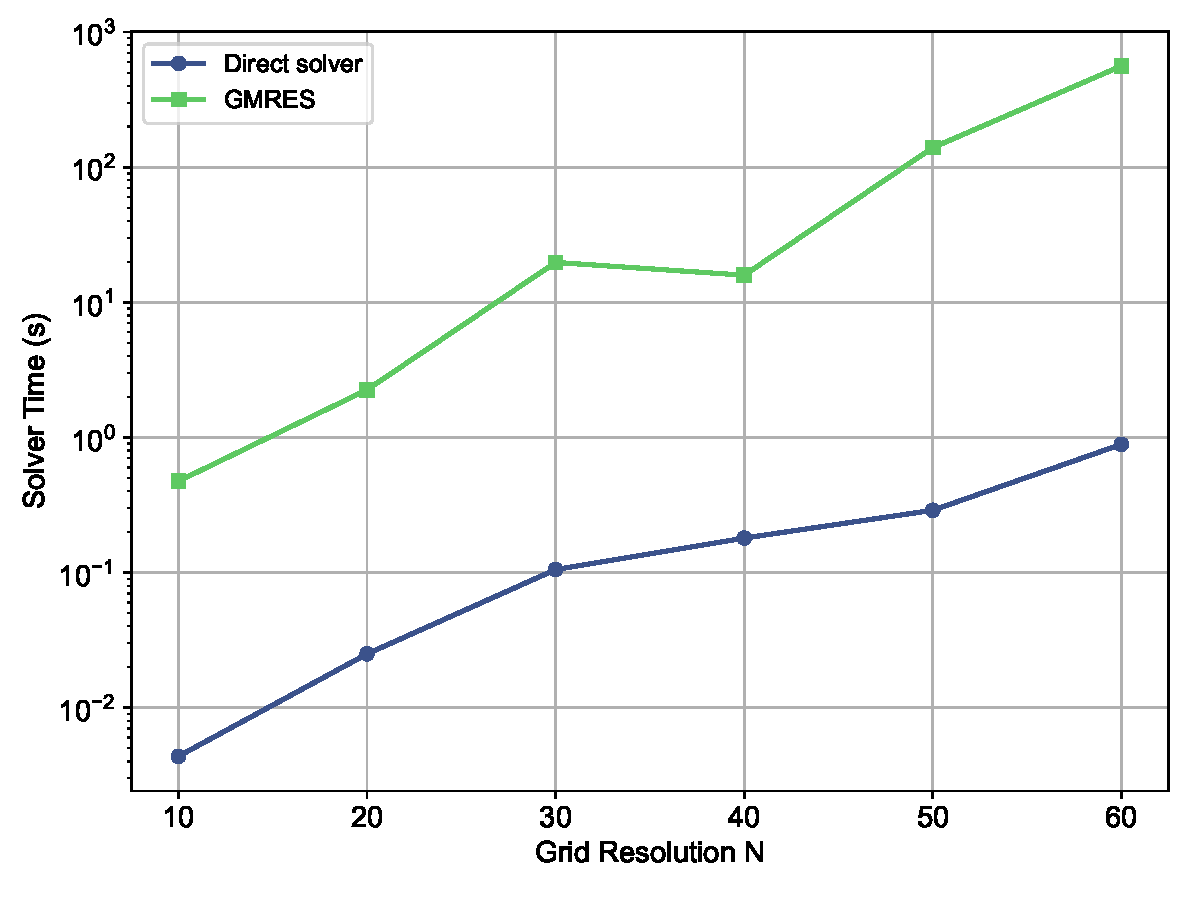
\includegraphics[width=0.8\textwidth]{gmres.pdf}
    \caption{Solution time for the direct sparse solver and GMRES at
    increasing grid resolutions.}
    \label{fig:gmres}
\end{figure}

Figure~\ref{fig:gmres} shows that both solution methods required more computational time as the grid size increased, but the direct solver was faster over the range of grid sizes I tested. 

\begin{table}[htbp]
  \centering
  \caption{Solver differences for increasing grid sizes}
  \label{tab:my_table}
  \begin{tabular}{| c | c | c | c |}
    \hline
    N & Direct Solver Time (s) & GMRES Time (s) & Solution Difference \\ [0.5ex] 
    \hline
    10 & $0.0044$ & $0.4743$ & $6.73e-02$ \\ 
    20 & $0.0250$ & $2.2511$ &  $4.23e-02$ \\ 
    30 & $0.1052$ & $19.7470$ & $2.87e-02$ \\ 
    40 & $0.1799$ & $15.8753$ &  $2.22e-02$ \\ 
    50 & $0.2889$ & $139.5089$ & $1.88e-02$ \\ 
    60 & $0.8885$ & $561.1151$ &  $1.73e-02$ \\ 
    \hline
  \end{tabular}
\end{table}

The relative difference between the GMRES and direct solver solutions decreased as the grid resolution increased, from 0.0673 for $N=10$ to 0.0173 for $N=60$. GMRES returned an info value of 0 for all grid sizes showing that it converged. The solutions were reasonably close. \\

Although GMRES was not faster than the direct solver for the grid sizes I tested, both methods produced similar numerical solutions. The results indicate that, for the grid sizes I tested, the direct solver was the more computationally efficient method.

\end{document}